%auto-ignore
\section{BERT 추가 세부 사항}
\label{appendix:sec:bert_description}



\begin{figure*}[ht]
\begin{center}
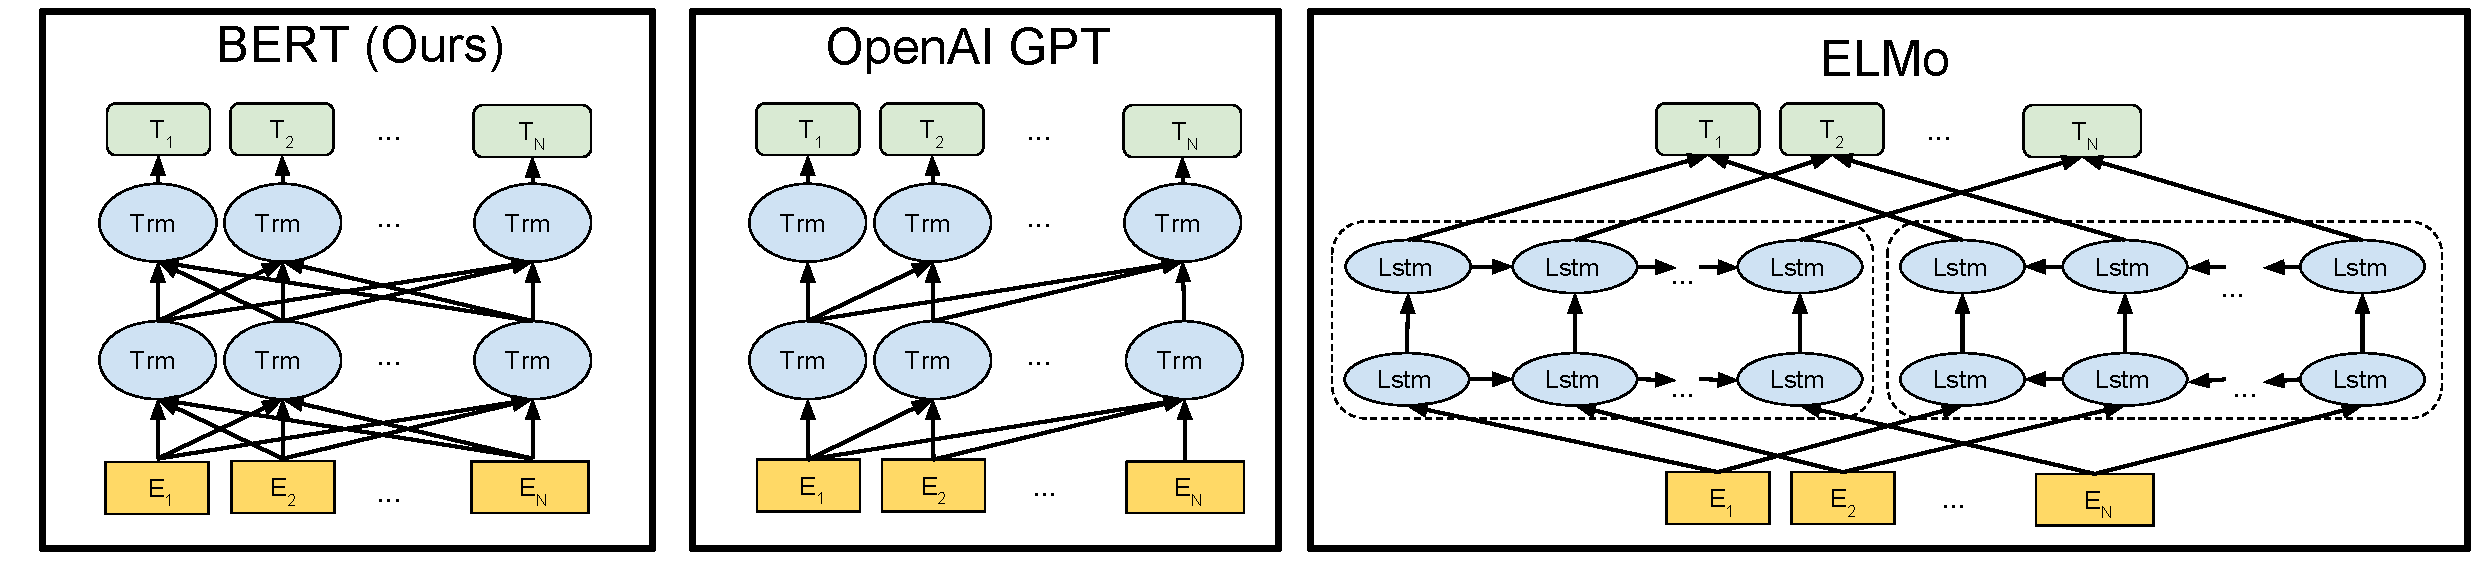
\includegraphics[width=\textwidth]{BERT_comparisons.pdf}
\end{center}
\caption{사전학습 모델 아키텍처의 차이. BERT는 양방향 트랜스포머를 사용한다. OpenAI GPT는 좌→우 트랜스포머를 사용한다. ELMo는 독립적으로 학습된 좌→우와 우→좌 LSTM의 결합을 사용해 다운스트림 과제용 피처를 생성한다. 셋 중에서, 모든 층에서 좌·우 맥락에 함께 조건화되는 표현을 만드는 것은 \bert뿐이다. 아키텍처 차이 외에, BERT와 OpenAI GPT는 파인튜닝 접근이고 ELMo는 피처 기반 접근이라는 차이도 있다.}
\label{fig:BERT_comparisons}
\end{figure*}


\subsection{사전학습 과제 예시}
다음에 사전학습 과제의 예시를 제공한다.

\paragraph{마스킹 LM과 마스킹 절차}

비라벨 문장이 {\tt {\small my dog is hairy}}이고, 무작위 마스킹 절차에서 4번째 토큰({\tt {\small hairy}}에 해당)을 선택했다고 가정하면, 마스킹 절차는 다음과 같이 더 자세히 표현될 수 있다.
\begin{itemize}
%\item Rather than {\em always} replacing the chosen words with {\tt [MASK]}, the data generator will do the following:
\item 80\,\% 확률로 단어를 {\tt [MASK]} 토큰으로 바꾼다 — 예: {\tt {\small my dog is hairy $\rightarrow$ my dog is [MASK]}}
\item 10\,\% 확률로 단어를 무작위 단어로 바꾼다 — 예: {\tt {\small my dog is hairy $\rightarrow$ my dog is apple}}
\item 10\,\% 확률로 단어를 그대로 둔다 — 예: {\tt {\small my dog is hairy $\rightarrow$ my dog is hairy}}. 그 목적은 표현이 실제 관측된 단어 쪽으로 편향되도록 만드는 것이다.
\end{itemize}

이 절차의 장점은, 트랜스포머 인코더가 어떤 단어를 예측하라고 요청받을지, 어떤 단어가 무작위 단어로 바뀌었는지를 미리 알 수 없다는 점이다. 따라서 인코더는 \emph{모든} 입력 토큰에 대한 분포적 맥락 표현을 유지하지 않을 수 없다. 또한 무작위 치환은 전체 토큰의 1.5\,\%(15\,\%의 10\,\%)에서만 일어나므로, 모델의 언어 이해 능력을 해치지는 않는 것으로 보인다. 이 절차의 영향은 \S\ref{appendix:sec:different_masks}에서 평가한다.

표준 언어모델 학습과 달리, 마스킹 LM은 각 배치에서 토큰의 15\,\%에 대해서만 예측을 수행한다. 이는 모델이 수렴하는 데 더 많은 사전학습 스텝이 필요할 수 있음을 시사한다. \S\ref{sec:num_training_steps}에서 저자들은 MLM이 모든 토큰을 예측하는 좌→우 모델보다 약간 느리게 수렴하지만, MLM의 경험적 향상이 늘어난 학습 비용을 훨씬 능가함을 보인다.

\paragraph{다음 문장 예측}

다음 문장 예측 과제는 다음 예시들로 표현될 수 있다.
\begin{align*}
\text{Input\;} &= \text{\tt {\scriptsize [CLS] the man went to [MASK] store [SEP]}} \\
& \text{\tt {\scriptsize \;\;\;\;\;\;\;he bought a gallon [MASK] milk [SEP]}}\\
\text{Label} &= \text{\tt {\scriptsize IsNext}} \\
\\
\text{Input\;} &= \text{\tt {\scriptsize [CLS] the man [MASK] to the store [SEP]}}\\
&\text{\tt {\scriptsize \;\;\;\;\;\;\;penguin [MASK] are flight \#\#less birds [SEP]}}\\
\text{Label} &= \text{\tt {\scriptsize NotNext}}
\end{align*}

\subsection{사전학습 절차}
\label{sec:pretraining_procedure}

각 학습 입력 시퀀스를 만들기 위해, 저자들은 코퍼스에서 두 개의 텍스트 구간을 샘플링한다 — 보통 단일 문장보다 훨씬 길지만(때로는 더 짧을 수도 있음) ``문장(sentences)''이라고 부른다. 첫 번째 문장은 {\tt A} 임베딩을, 두 번째는 {\tt B} 임베딩을 받는다. 50\,\% 확률로 {\tt B}는 {\tt A} 뒤에 실제로 따라오는 다음 문장이고, 50\,\% 확률로 무작위 문장이며, 이는 ``다음 문장 예측'' 과제용으로 만들어진다. 결합 길이가 512 토큰 이하가 되도록 샘플링한다. LM 마스킹은 WordPiece 토큰화 이후에 일률적인 15\,\% 마스킹 비율로 적용되며, 부분 단어 조각에 대한 특별 고려는 두지 않는다.

저자들은 256 시퀀스(256 시퀀스 × 512 토큰 = 128,000 토큰/배치) 배치 크기로 1,000,000 스텝 동안 학습하며, 이는 33억 단어 코퍼스 위에서 약 40 에포크에 해당한다. 학습률 1e-4의 Adam을 사용하고, ${\beta}_1=0.9$, ${\beta}_2=0.999$, L2 가중치 감쇠 $0.01$, 첫 10,000 스텝에 대한 학습률 워밍업, 그리고 학습률의 선형 감쇠를 적용한다. 모든 층에 0.1 확률의 드롭아웃을 사용한다. OpenAI GPT를 따라 표준 {\tt relu} 대신 {\tt gelu} 활성을 사용한다~\cite{hendrycks:2016}. 학습 손실은 평균 마스킹 LM 우도와 평균 다음 문장 예측 우도의 합이다.

\bertbase의 학습은 Pod 구성의 4 Cloud TPU(총 16 TPU 칩)에서 수행되었다.\footnote{https://cloudplatform.googleblog.com/2018/06/Cloud-TPU-now-offers-preemptible-pricing-and-global-availability.html} \bertlarge의 학습은 16 Cloud TPU(총 64 TPU 칩)에서 수행되었다. 각 사전학습은 완료까지 4일이 걸렸다.

어텐션이 시퀀스 길이의 이차 함수이므로 더 긴 시퀀스는 비용이 불균형하게 크다. 실험에서 사전학습 속도를 높이기 위해, 저자들은 전체 스텝의 90\,\%를 시퀀스 길이 128로 사전학습한 뒤, 나머지 10\,\%를 시퀀스 길이 512로 학습해 위치 임베딩을 학습시킨다.

\subsection{파인튜닝 절차}
파인튜닝에서는 배치 크기, 학습률, 학습 에포크 수를 제외하면 대부분의 모델 하이퍼파라미터가 사전학습과 동일하다. 드롭아웃 확률은 항상 0.1로 유지했다. 최적 하이퍼파라미터 값은 과제별로 다르지만, 저자들은 모든 과제에서 다음 범위의 값들이 잘 작동함을 확인했다.

\begin{itemize}[noitemsep]
\item {\bf 배치 크기}: 16, 32
\item {\bf 학습률 (Adam)}: 5e-5, 3e-5, 2e-5
\item {\bf 에포크 수}: 2, 3, 4
\end{itemize}

또한 큰 데이터셋(예: 라벨 학습 예시 100k+)이 작은 데이터셋보다 하이퍼파라미터 선택에 훨씬 덜 민감하다는 점도 관찰했다. 파인튜닝은 보통 매우 빠르므로, 위 파라미터들에 대해 단순한 전수 탐색을 돌리고 개발 셋 성능이 가장 좋은 모델을 고르는 것이 합리적이다.

\subsection{BERT, ELMo, OpenAI GPT 비교}
\label{appendix:sec:comparing_bert_and_openai}

여기서는 ELMo, OpenAI GPT, BERT를 포함한 최근 대표 표현 학습 모델들의 차이를 살핀다.
모델 아키텍처 사이의 비교는 그림~\ref{fig:BERT_comparisons}에 시각적으로 정리되어 있다. 아키텍처 차이 외에도, BERT와 OpenAI GPT는 파인튜닝 접근이고 ELMo는 피처 기반 접근이라는 점에 유의한다.

BERT와 가장 비교 가능한 기존 사전학습 방법은 OpenAI GPT다. GPT는 큰 텍스트 코퍼스에서 좌→우 트랜스포머 LM을 학습한다.
사실 BERT의 많은 설계 결정은 두 방법을 최소한의 차이로 비교할 수 있도록, GPT와 가능한 한 가까워지도록 의도적으로 내려진 것이다.
본 연구의 핵심 주장은 \S\ref{sec:pretraining_tasks}에 제시된 양방향성과 두 사전학습 과제가 경험적 향상의 대부분을 설명한다는 것이지만, BERT와 GPT의 학습 방식 사이에는 다음과 같은 다른 차이도 있음을 언급한다.

\begin{itemize}
\item GPT는 BooksCorpus(800M 단어)로 학습된다. BERT는 BooksCorpus(800M 단어)와 Wikipedia(2,500M 단어)로 학습된다.
\item GPT는 파인튜닝 시점에만 도입되는 문장 분리자({\tt [SEP]})와 분류 토큰({\tt [CLS]})을 사용한다. BERT는 사전학습 동안 {\tt [SEP]}, {\tt [CLS]}, 그리고 문장 {\tt A}/{\tt B} 임베딩을 함께 학습한다.
\item GPT는 32,000 단어 배치 크기로 1M 스텝 동안 학습되었다. BERT는 128,000 단어 배치 크기로 1M 스텝 동안 학습되었다.
\item GPT는 모든 파인튜닝 실험에 동일한 학습률 5e-5를 사용했다. BERT는 개발 셋 성능이 가장 좋은 과제별 파인튜닝 학습률을 선택한다.
\end{itemize}

이런 차이의 효과를 분리하기 위해, 저자들은 \S\ref{sec:task_ablation}에서 절제 실험을 수행해 향상의 대부분이 실제로 두 사전학습 과제와 이들이 가능하게 하는 양방향성에서 비롯됨을 입증한다.



\subsection{서로 다른 과제에 대한 파인튜닝 도식}
\label{appendix:sec:fine_tune_details_and_figures}

서로 다른 과제에 대해 BERT를 파인튜닝하는 도식은 그림~\ref{fig:bert_fine_tune}에서 볼 수 있다. 저자들의 과제별 모델은 \bert에 출력 층 하나를 추가해 만들기 때문에, 처음부터 학습해야 하는 파라미터 수가 최소화된다. 이 과제들 중 (a)와 (b)는 시퀀스 수준 과제이고, (c)와 (d)는 토큰 수준 과제다. 그림에서 $E$는 입력 임베딩, $T_i$는 토큰 $i$의 맥락 표현, \textsc{[CLS]}는 분류 출력의 특수 기호, \textsc{[SEP]}는 비연속 토큰 시퀀스를 분리하는 특수 기호다.
\begin{figure*}[ht]
\begin{center}
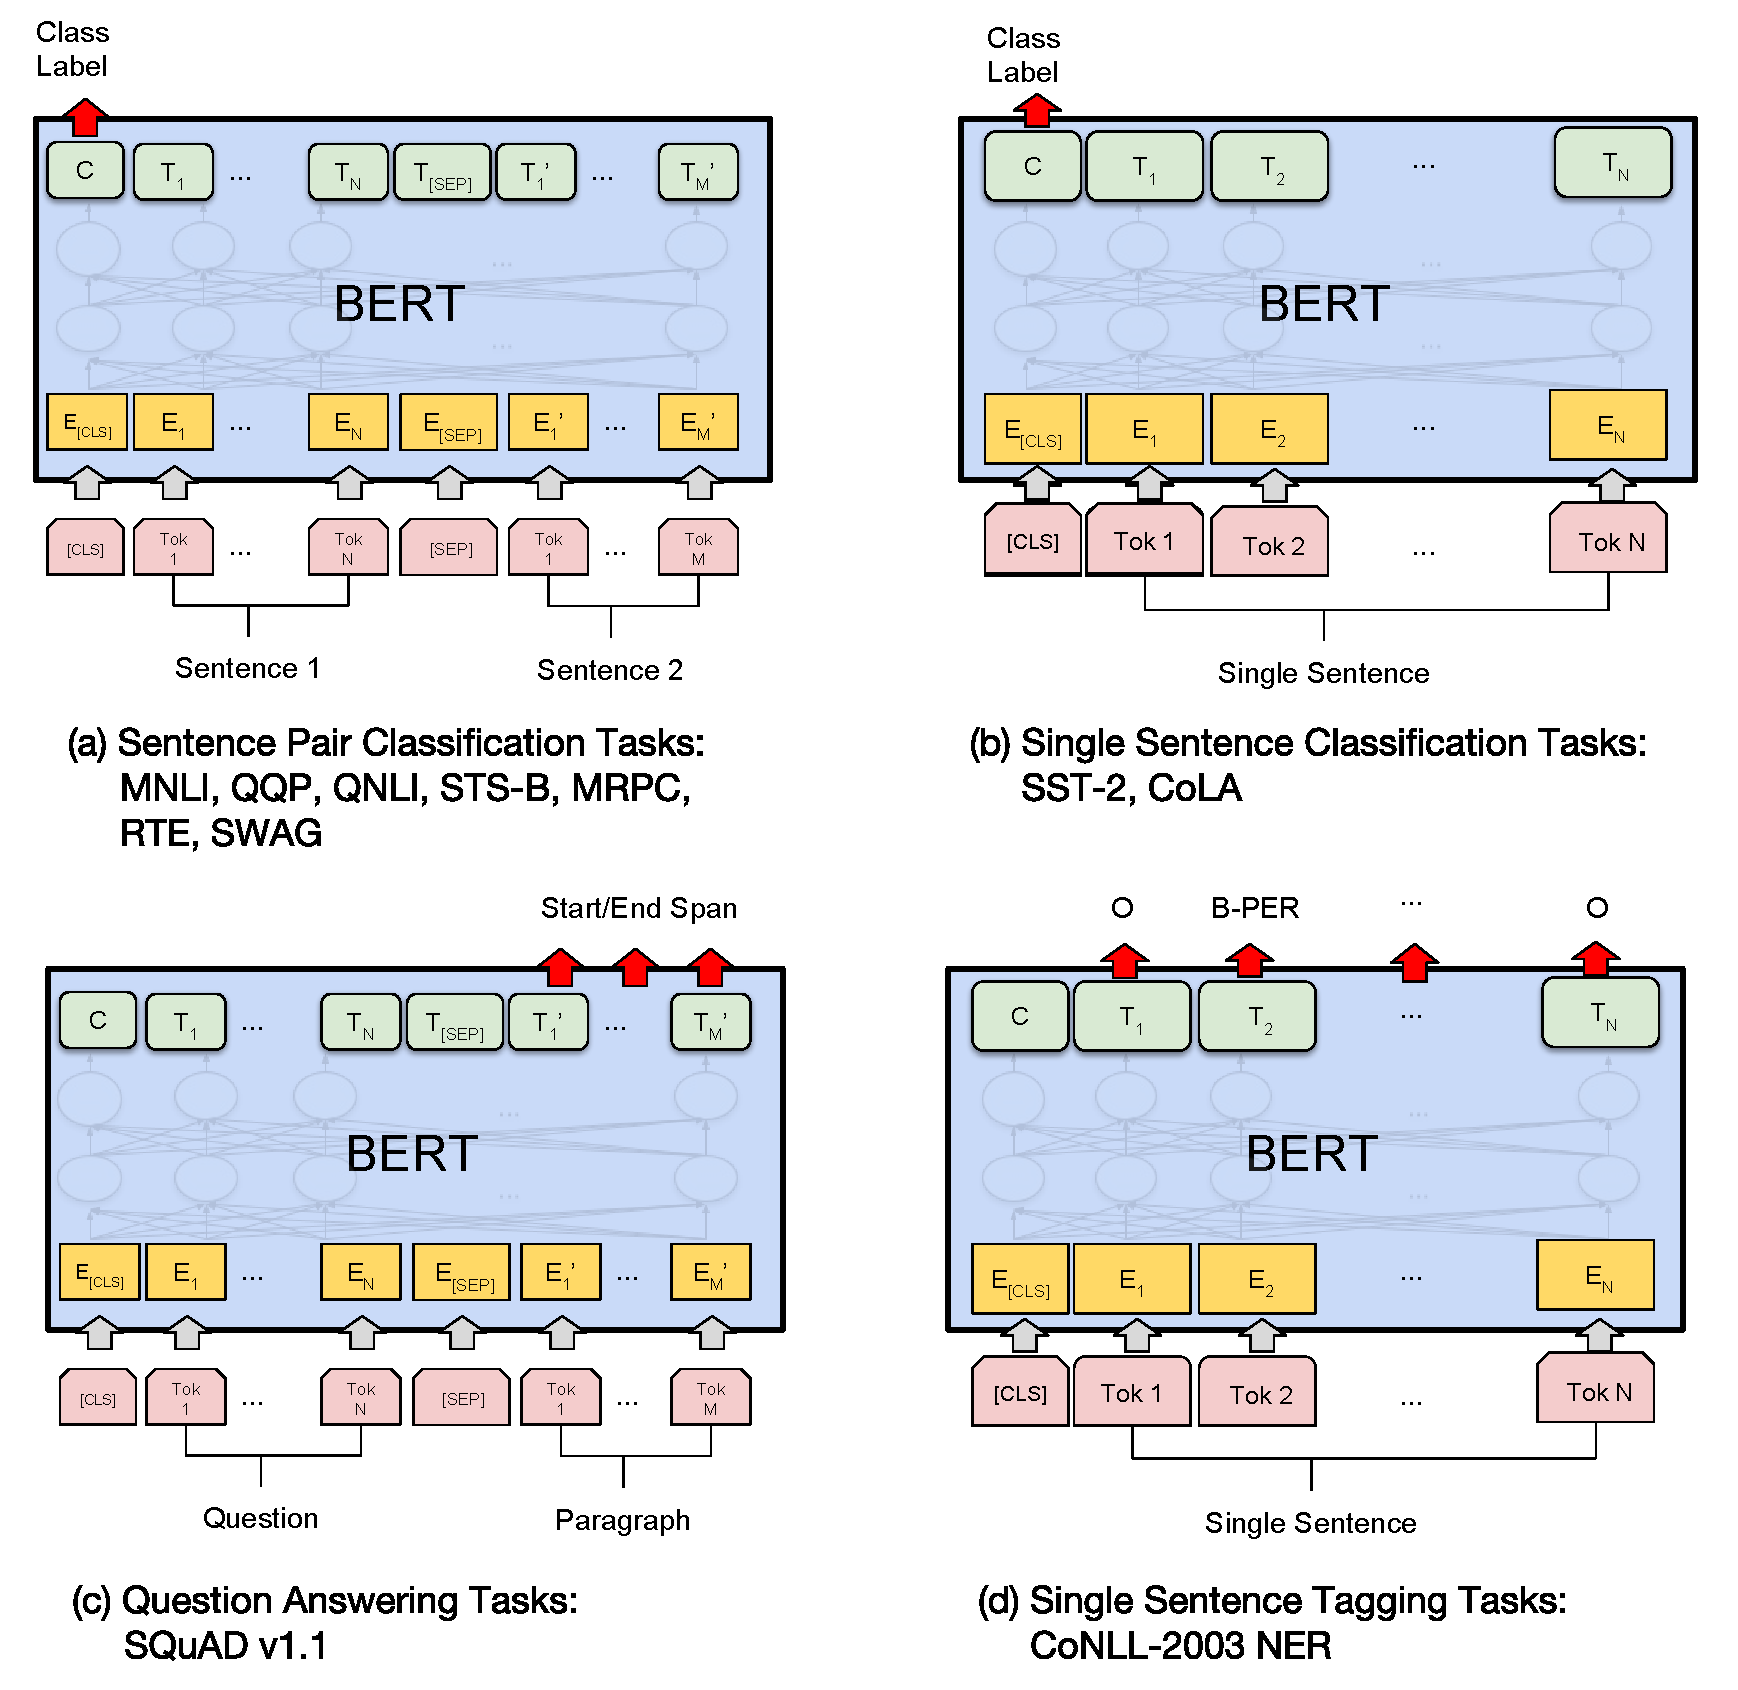
\includegraphics[width=0.85\textwidth]{BERT_fine_tune.pdf}
\end{center}
\caption{서로 다른 과제에 대한 BERT 파인튜닝 도식.}
\label{fig:bert_fine_tune}
\end{figure*}




